\documentclass[11pt,a4paper]{article} 
\usepackage[utf8]{inputenc}
\usepackage[T1]{fontenc}
\usepackage{amsmath,amsfonts,amssymb} 
\usepackage{booktabs} 
\usepackage{float} 
\usepackage{enumitem}
\usepackage{graphicx}
\usepackage{multirow}

\usepackage[margin=2cm]{geometry} 

\title{\vspace{-0.5cm}\textbf{Security Analysis and Phishing Classification of Websites}}
\author{Name and Surname}
\date{May 25, 2026} 

\begin{document}

\maketitle 

\begin{abstract}
\noindent This report presents a comprehensive security analysis and classification of the ``Website Phishing'' dataset, originally collected from the Internet by cybersecurity specialists. The primary objective is to evaluate technical and behavioral website attributes to distinguish between legitimate and malicious entities. First, an exploratory data analysis was conducted to investigate key statistical properties, including variance, covariance and correlation coefficients. Next, a Support Vector Machine (SVM) classification model was implemented to predict phishing threats. Finally, the classification performance was visualized and subjected to a critical discussion.
\end{abstract}

\section{(a) Statistical Analysis and Data Summary}
The dataset chosen for this report consists of $N = 1082$ records and 10 numerical features. Collected features hold the categorical values Legitimate, Suspicious, Phishing, these values have been replaced with numerical values 1, 0, -1 respectively.

\begin{description}[itemsep=1pt, topsep=2pt, parsep=1pt]
    \item[SFH] (Server Form Handler) - measures the destination of user-submitted form data.
    \item[popUpWindow] - checks if a malicious pop-up window is displayed asking for confidential information.
    \item[SSLfinal\_State] - indicate whether the SSL certificate is being used correctly.
    \item[Request\_URL] - track the proportion of external objects and links pointing out of the home domain.
    \item[URL\_of\_Anchor] - measures the percentage of the hyperlink inside the html tags that point to the external domains.
    \item[web\_traffic] - popularity of the site.
    \item[URL\_Length] - checks the URL length, whether it is too long or has a good length.
    \item[age\_of\_domain] - domain existence period.
    \item[having\_IP\_Address] - checks whether a raw IP address is used in the URL instead of a standard domain name.
    \item[Result] - tells if the site is Legitimate (1), Suspicious (0), Phishing (-1).
\end{description}

\vspace{0.2cm} 

\begin{table}[H] 
\centering
\caption{Descriptive statistics for the web attributes ($N = 1082$).}
\label{tab:descriptive_stats}
\begin{tabular}{lccccc}
\toprule
\textbf{Feature} & \textbf{Min} & \textbf{Mean} & \textbf{Median} & \textbf{Max} & \textbf{Variance} \\
\midrule
SFH                 & -1 &  0.2523 &  1 & 1 & 0.8382 \\
popUpWindow         & -1 & -0.2606 &  0 & 1 & 0.4574 \\
SSLfinal\_State     & -1 &  0.3420 &  1 & 1 & 0.6637 \\
Request\_URL        & -1 & -0.2366 &  0 & 1 & 0.6341 \\
URL\_of\_Anchor      & -1 & -0.0471 &  0 & 1 & 0.8701 \\
web\_traffic        & -1 &  0.0083 &  0 & 1 & 0.6632 \\
URL\_Length         & -1 & -0.0518 &  0 & 1 & 0.5857 \\
age\_of\_domain      & -1 &  0.2237 &  1 & 1 & 0.9509 \\
having\_IP\_Address   &  0 &  0.1081 &  0 & 1 & 0.0965 \\
Result              & -1 & -0.1192 & -1 & 1 & 0.9025 \\
\bottomrule
\end{tabular}
\end{table}

Looking at the table, we can see basic statistics. The most important here is the \textbf{Mean}, which shows us how the data are distributed and whether -1, 0, or 1 is the dominant value. Based on this, we can deduce that hackers have big problems with \textbf{SSL} and \textbf{age\_of\_domain}—these are clearly their technical weak points. The mean of the results also shows that in our training data, we have a higher proportion of Phishing websites. 
The rest of the statistics do not tell us much more about the data because we only use -1, 0, and 1. Variance and Median do not operate well with these discrete, opposite numbers. The Min and Max values only show that we use 3 numbers for the classification (or 2, like in \textbf{having\_IP\_Address}).

What is more interesting is shown in the covariance matrix and correlation matrix. \textbf{web\_traffic} has a strong inverse correlation with \textbf{age\_of\_domain} and a relatively good connection with the final \textbf{Result}. What is really interesting here is that the data perfectly shows how hackers operate—they often have to buy an old, expired domain to hide their true target and bypass security filters, even if that domain currently lacks active traffic. Moreover, \textbf{SFH}, \textbf{popUpWindow}, and \textbf{SSLfinal\_State} show us that if those three features are too suspicious, the \textbf{Result} is heavily shifted towards Phishing (-1). In this case, the covariance matrix shows highly convergent data to the correlation matrix, so there is no need to analyze both. They display the same patterns simply because all of our variables are strictly limited to the scale from -1 to 1.

\section{(b) Support Vector Machine Classification}
The Support Vector Machine (SVM) algorithm was selected due to the low dimensionality of the dataset, which consists of exactly 9 features. SVM is exceptionally well-suited for this scale of data, minimizing the risk of the ``curse of dimensionality'' and leading to robust generalisation and better predictions. Since the data exhibits non-linear relationships, a Support Vector Classifier with a Radial Basis Function (RBF) kernel was applied. The decision function of this model is defined as follows:

\begin{equation}
f(x) = \text{sign} \left( \sum_{i \in SV} \alpha_i y_i \exp(-\gamma \|x - x_i\|^2) + b \right)
\label{eq:svm_rbf}
\end{equation}

For the experimental setup, the dataset was partitioned into a training set (80\%) and a testing set (20\%). The model was trained exclusively on the 80\% subset, while the remaining 20\% was reserved to evaluate the model's predictive performance on unseen data.

At first glance, the overall accuracy of 90.41\% might seem merely good, rather than outstanding. However, the most critical insights lie within the confusion matrix. The matrix reveals that nearly half of the total mistakes are False Positives, meaning the model incorrectly flags a legitimate website as phishy. In a cybersecurity context, this type of error is acceptable; blocking a user from a safe site causes minor inconvenience, but it is far less dangerous than committing a False Negative, which would allow a malicious phishing site to pass through undetected.

\section{(c) Results Visualization and Critical Discussion}
The visual representation of the model's performance on the 20\% test dataset is illustrated in the confusion matrix heatmap below (Figure~\ref{fig:svm_confusion}).

\begin{figure}[H]
    \centering
    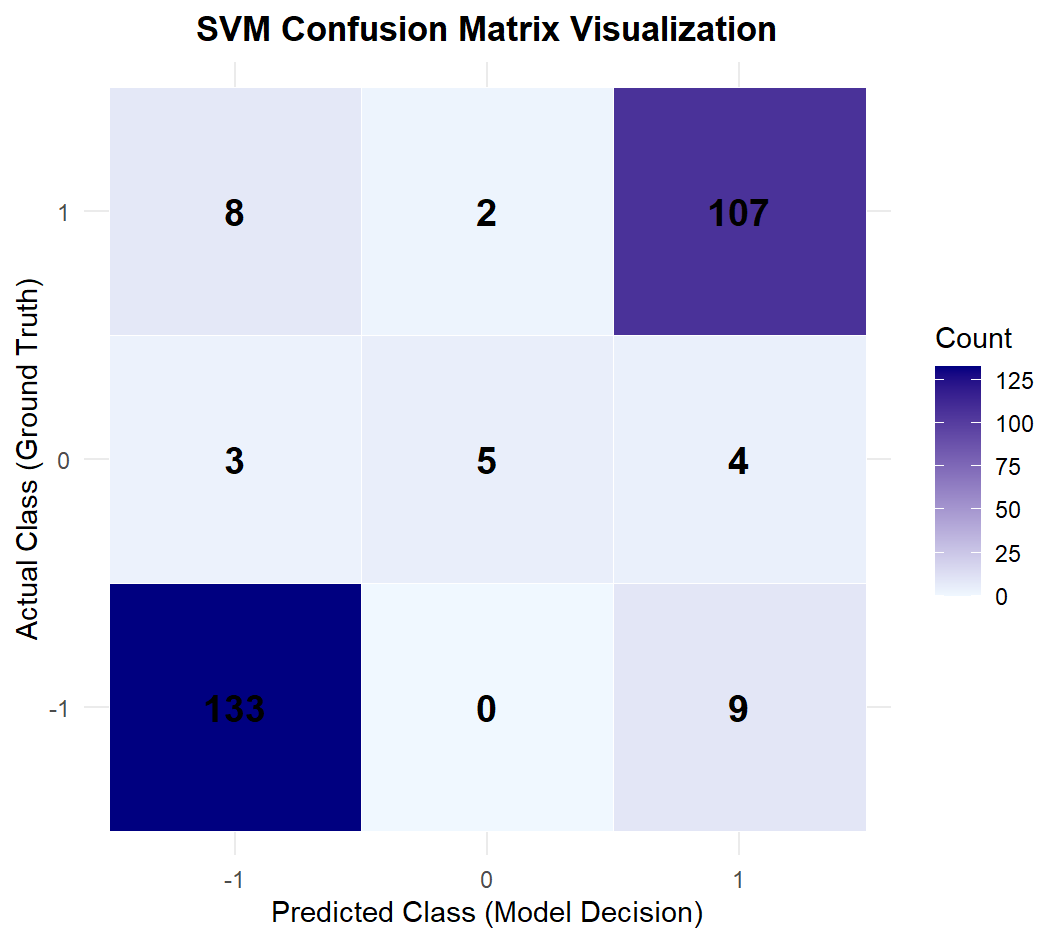
\includegraphics[width=0.65\textwidth]{Rplot02.png} 
    \caption{Heatmap Visualization of the SVM Confusion Matrix.}
    \label{fig:svm_confusion}
\end{figure}

To provide a comprehensive evaluation of the applied Support Vector Machine method on this website phishing dataset, several critical advantages and disadvantages must be discussed:

\subsection*{Advantages:}
\begin{itemize}[itemsep=1pt, topsep=2pt]
    \item \textbf{Efficiency with Low Dimensionality:} With exactly 9 input features, SVM efficiently constructs an optimal separating boundary without suffering from high computational complexity.
    \item \textbf{Nonlinear Flexibility:} The Radial Basis Function (RBF) kernel allows the algorithm to effortlessly map complex, nonlinear interactions between technical attributes into a higher-dimensional space where they become separable.
    \item \textbf{Generalisation Capacity:} The soft-margin formulation ($C=1$) prevents overfitting to noise in the training set, allowing the model to remain robust when evaluated on unseen test instances.
\end{itemize}

\subsection*{Disadvantages:}
\begin{itemize}[itemsep=1pt, topsep=2pt]
    \item \textbf{Lack of Interpretability:} SVM functions primarily as a ``black box'' model. Unlike decision trees, it does not output straightforward rules, making it difficult to explain to an end-user exactly why a specific URL was flagged.
    \item \textbf{Sensitivity to Hyperparameters:} The classification performance heavily relies on parameters such as $\gamma$ and $C$. Achieving optimal results requires extensive tuning, as poor parameter selection can significantly degrade accuracy.
    \item \textbf{Sensitivity to Class Ambiguity:} The model struggled significantly with the intermediate ``Suspicious (0)'' category, misclassifying a high proportion of those samples due to overlapping geometric characteristics with the other two classes.
\end{itemize}

\end{document}